\documentclass[11pt, oneside]{article}   	% use "amsart" instead of "article" for AMSLaTeX format
\usepackage[margin=1in]{geometry}               % See geometry.pdf to learn the layout options. There are lots.
\geometry{letterpaper}                   	% ... or a4paper or a5paper or ... 
%\geometry{landscape}                		% Activate for rotated page geometry
%\usepackage[parfill]{parskip}    		% Activate to begin paragraphs with an empty line rather than an indent
\usepackage{graphicx}				% Use pdf, png, jpg, or eps§ with pdflatex; use eps in DVI mode
						% TeX will automatically convert eps --> pdf in pdflatex		
\usepackage{amssymb}
\usepackage{amsmath}
\usepackage{array}
\usepackage{indentfirst}
\usepackage{enumitem}
\usepackage{mathptmx}
\usepackage{float}

%SetFonts

%SetFonts

\setcounter{secnumdepth}{3} % default value for 'report' class is "2"

\title{APPM 4560 Laboratory 1 Report}
\author{Rhys Olsen\\
\texttt{rhys.olsen@colorado.edu}
 \and Jessica Petty\\
 \texttt{jessica.petty@colorado.edu}
 }
\date{September 26, 2016}

\begin{document}
\maketitle
\section{Simulating Random Permutations}
\subsection{Simulating One Random Permutation}

Given the size-increasing ordered list of the finite set consisting of natural numbers $\left\{1, \dots, \right\}$ for some $n \in \mathbb{N}$, the following algorithm will simulate a random permutation of the list:

%Algorithm to Generate Random Permutation 

\subsubsection{Algorithm to Generate Random Permutation}\label{sssec:perm}
\begin{enumerate}[leftmargin=30pt,labelindent=65pt,itemindent=30pt]
\item[\textsc{step 1:}] Simulate and store $n$ random variables $U_1, \dots, U_n \sim \text{Uniform}(0,1)$

\item[\textsc{step 2:}] Define some $f$ that maps each $\text{Uniform}\left(0,1 \right)$ random variable to the index at which it was created

\item[\textsc{step 3:}] Order the $\text{Uniform}\left(0,1 \right)$ random variables in decreasing order

\item[\textsc{step 4:}] Apply $f$ to each $U_i$ to produce the permutation of integers
\end{enumerate}

\subsubsection{Probability of Observing a Fixed Permutation}
Fix a particular permutation $\sigma = (f(1), \dots, f(n))$ of the ordered list $\left\{1, \dots, n\right\}$ and consider a given random permutation generated according to~\ref{sssec:perm}. In general, having already selected the first $i$ numbers in a permutation to match the first $i$ of $\sigma$, the equal likelihood of any remaining number being next in the permutation implies that the probability the $i + 1$th number in the permutation will match the $i + 1$th of $\sigma$ is $\frac{1}{n - i}$. Conditioning on each successive number of the permutation matching $\sigma$ means that the probability of a randomly generated permutation matching $\sigma$ is:
\begin{equation}\label{eqn:fix}
  p_{\text{fixed}} = \frac{1}{n} \times \frac{1}{n - 1} \times \dots \times \frac{1}{1} = \frac{1}{n!}
\end{equation}

\subsection{\textit{X}: Number of Random Observations of a Particular Permutation}\label{ssec:x}
We define the random variable $X$ to be the number of random permutations of $\left\{1, \dots, n\right\}$ that equal $\sigma$ among $m$ such permutations generated by~\ref{sssec:perm}. Observe that the $m$ randomly generated permutations are independent. Since each permutation matches $\sigma$ with probability $p_{\text{fixed}} = \frac{1}{n!}$, we can treat $X$ as the number of successes among $m$ independent trials where a given success occurs with probability $p_{\text{fixed}}$. Under this treatment, the random variable $X$ therefore has a \textit{binomial} distribution with trial count $m$ and success probability $p_{\text{fixed}} = \frac{1}{n!}$. For the simulation of $X$ discussed in following sections, we are experimentally interested in the values $m = 6000$ and $n = 7$. Now, given that \textit{X} has a \textit{binomial} distribution, we seek its probability mass function $f_X(x)$ and expectation $\mathbb{E}[X]$.

To generalize, for $B \sim \text{Binomial}(n, p)$, of which $X$ is a particular case, we seek $f_B(k) = P(B = k)$, which we know is $f_B(k) = {n \choose k}p^k(1-p)^{n-k}, 0 \leq k \leq n$, which for $X$ with $m = 6000$ and $n = 7$ is $f_X(k) = {6000 \choose k}(\frac{1}{7!})^k(1-\frac{1}{7!})^{m-k} = {6000 \choose k}(\frac{1}{5040})^k(1-\frac{1}{5040})^{6000-k}$. Additionally, we know that $\mathbb{E}[B] = np$. Noting that, for this simulation, $X \sim \text{Binomial}(m,\frac{1}{n!})$, $\mathbb{E}[X] = \frac{m}{n!}$. For the constants $m = 6000$ and $n = 7$, this is $\mathbb{E}[X] = \frac{6000}{7!} = \frac{6000}{5040} = \frac{25}{21} \approx 1.19$.

\subsection{\textit{Y}: Number of Random Permutations Needed To Match A Particular Permutation}
We define the random variable $Y$ to be the number of random permutations of $\left\{1, \dots, n\right\}$ generated by~\ref{sssec:perm} needed to witness $\sigma$ once among the permutations. As was the case in \ref{ssec:x}, $Y$ can be described in terms of independent trials each succeeding with probability $p_{\text{fixed}} = \frac{1}{n!}$. In contrast to the random varaible $X$, however, the random variable $Y$ represents the number of independent trials that succeed with probability $p_{\text{fixed}}$ needed for the last trial to be a success. Under this characterization, $Y$ is a \textit{geometric} random variable with success probability $p_{\text{fixed}}$. We seek its probability mass function $f_Y(y)$ and expectation $\mathbb{E}[Y]$. For the simulation of $Y$ mentioned in sections to follow, we are experimentally interested in the value of $n = 7$.

A geometric random variable $G \sim \text{Geometric}(p)$ has probability density function $f_G(k) = p(1-p)^{k-1}, 1 \leq k < \infty$. Since $Y \sim \text{Geometric}(\frac{1}{n!})$, $f_Y(y) = \frac{1}{n!} * (1 - \frac{1}{n!})^{y-1}, 1 \leq k < \infty$. For $n = 7$, this is $f_Y(y) = \frac{1}{7!} * (1 - \frac{1}{7!})^{y-1} = \frac{1}{5040} * (1 - \frac{1}{5040})^{y-1}, 1 \leq k < \infty$.

Additionally, because $Y \sim \text{Geometric}$, we know that $\mathbb{E}[Y] = \frac{1}{p}$. As a consequence, for this simulation we have $\mathbb{E}[Y] = \frac{1}{1/n!} = n!$, where again $n$ gives the upper bound on the set $\{1, \dots, n\}$ being permuted. For $n = 7$, this is $\mathbb{E}[Y] = 7! = 5040$.

\subsection{Comparison of Theoretical Distribution of \textit{X} With Simulation}

% \begin{figure}[H]
\begin{figure}
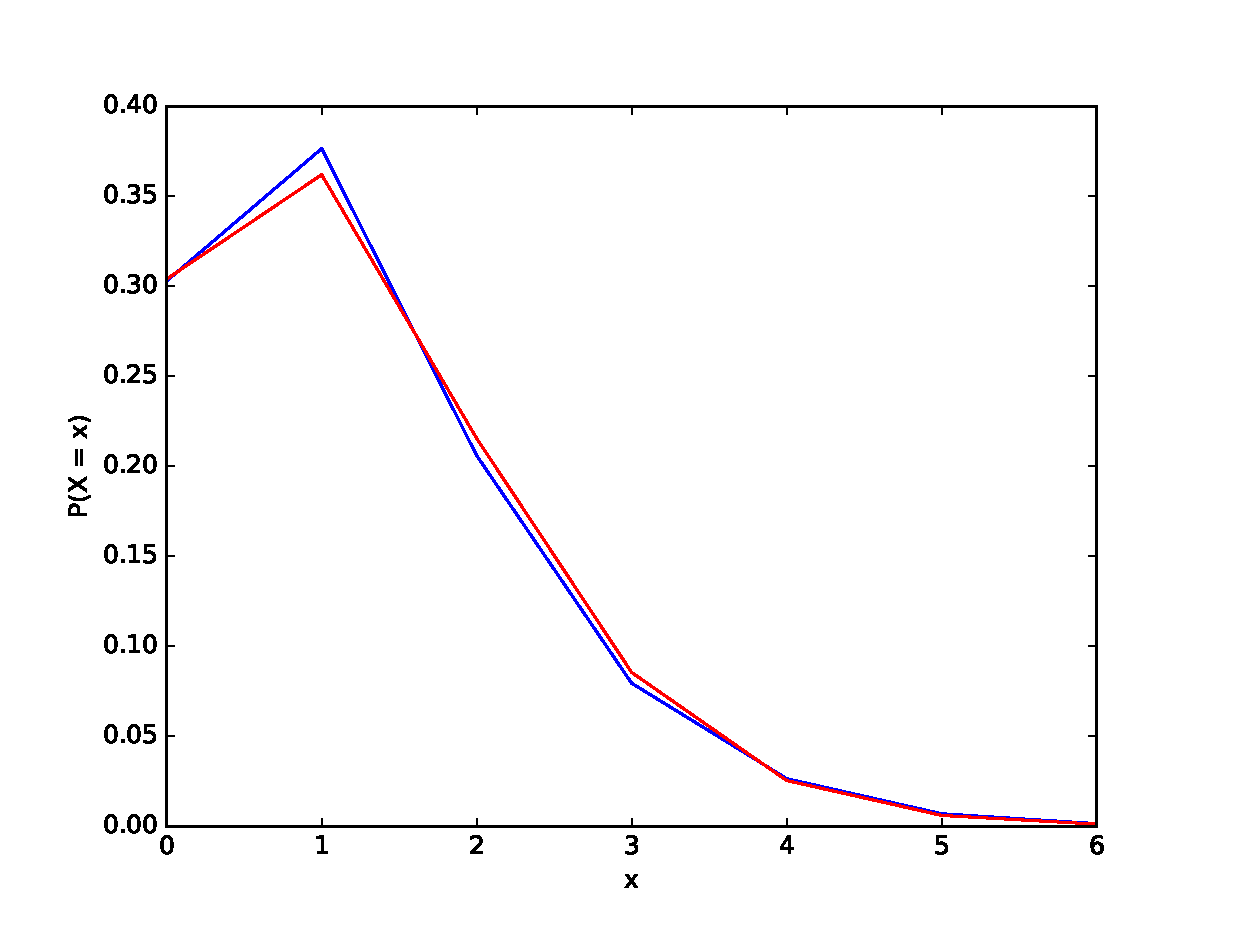
\includegraphics[scale=.5]{part_1_problem_4}
\caption{Plot of likelihood versus support value of the random variable $X$ with $m = 6000$ and $n = 7$ for $k = 2000$ computer simulations of the random variable (in blue) compared with the theoretical distribution that $X$ respects (in red). Note that the computer simulations have been normalized such that the sum of the histogram bins is $1$. Notice that the experimental plot is quite similar to the theoretical one, with slightly less variance.}
\label{fig:x}
\end{figure}
%Plot of likelihood versus support value of the random variable $X$ with $m = 6000$ and $n = 7$ for $k = 2000$ computer simulations of the random variable (in blue) compared with the theoretical distribution that $X$ respects (in red). Note that the computer simulations have been normalized such that the sum of the histogram bins is $1$. Notice that the experimental plot is quite similar to the theoretical one, with slightly less variance.

We implement a procedure to simulate $X$ with $m = 6000$ and $n = 7$ by generating $m$ permutations using the algorithm given in \ref{sssec:perm} and counting the number of those $m$ permutations that equal $\sigma = (6, 7, 2, 5, 1, 4, 3)$. Using this procedure, We simulate $X$ $k = 2000$ times and plot its histogram against the theoretical distribution for $X$ in figure~\ref{fig:x}. Our plot shows strong agreement between the theoretical distribution and its simulation, suggesting that both the analysis of the random variable $X$ and the implementation of the simulation are correct.

\subsection{Comparison of Theoretical Distribution of \textit{Y} With Simulation}

\begin{figure}
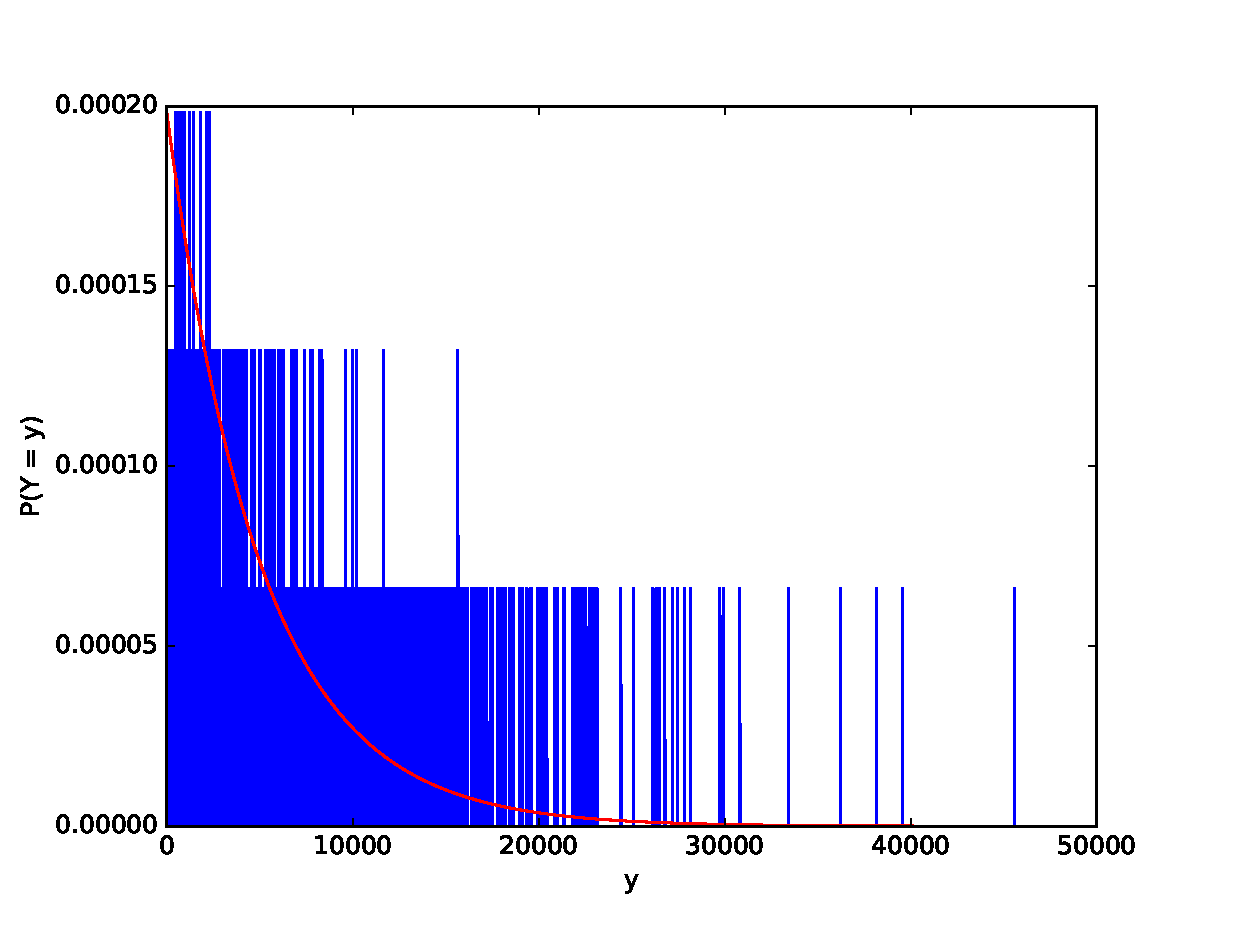
\includegraphics[scale=.5]{part_1_problem_5}
\caption{Plot of likelihood versus support value of the random variable $Y$ with $n = 7$ for $k = 2000$ computer simulations of the random variable (in blue) compared with the theoretical distribution that $X$ respects (in red). Note that the computer simulations have been normalized such that the tallest of the histogram bins is equal in height to the mode value of the geometric model, which is at $Y = 1$. While it's less obvious than in figure~\ref{fig:x} that the simulations agree with the theoretical model due to how simulating $Y$ $k = 2000$ times samples the larger support more sparsely and results in very low counts of each measured event, the density of the blue lines in any given horizontal region and simulation sample count threshold agrees with the proportion of blue in the same horizontal region and sample count threshold that is below the red line representing the probability density function.}
\label{fig:y}
\end{figure}

We implement a procedure to simulate $Y$ with $n = 7$ by generating permutations using the algorithm given in \ref{sssec:perm}, keeping a count of how many random permutations we generate, and returning this count as soon as a permutation is generated that equals $\sigma = (6, 7, 2, 5, 1, 4, 3)$. Using this procedure, We simulate $Y$ $k = 2000$ times and plot its histogram against the theoretical distribution for $Y$ in figure~\ref{fig:y}. Once again, our plot shows strong agreement between the theoretical distribution and its simulation, inspiring confidence in the correctness of our analysis and simulation.

\section{Computing Performance of Retrieving Algorithms}
\subsection{Method A: Linear search}
We define method A for retrieving as follows: to search a permutation for a given value (in this case, 1), iterate through the values from first to last until 1 is found. Let the random variable $Q_A$ denote the number of times needed to search the permutation until 1 is found. We seek $\mathbb{E}[Q_A]$.

$Q_A$'s probability mass function $f_{Q_A}(x)$ represents the probability of position $x$ being the location of the number 1. Note that each possible position of the number 1 is equally likely with probability $1 / n$, so $f_{Q_A}(x) = 1 / n, 1 \leq x \leq n$. This means $\mathbb{E}[Q_A] = \sum_{k=1}^{n} \frac{1}{n} k = \frac{1}{n} \sum_{k = 1}^{n} k = \frac{1}{n} \frac{n (n + 1)}{2} = \frac{n + 1}{2}$.
\subsection{Simulating Method A}
Using the algorithm given in \ref{sssec:perm}, we simulate $Q_A$ on ten thousand random permutations and determined the sample average of $Q_A$ for each permutation size $n$ drawn from the set $\left\{9, 21, 36, 69\right\}$. A table of these values compared with our theoretical expectation is included in the next section.

\subsection{Result of Simulation of Method A Compared With Theory}
The following table summarizes the simulation of $Q_{A}$ for various permutation lengths and compares this simulation with the theoretical expected values for $Q_{A}$:\\

\begin{tabular} {| m{4cm} || m{3cm} | m{3cm} || m{3.5cm} |}
\hline
\multicolumn{4} {| c |} {Comparison of Theoretical and Simulated Averages for $Q_{A}$}\\
\hline\hline
Permutation Length & Simulated & Theoretical : $\frac{n + 1}{2}$ & Percent Error\\
\hline
$n=9$  & 5.0246  & 5    & 0.492\%  \\
$n=21$ & 10.92   & 11   & 0.727\%  \\
$n=36$ & 18.6098 & 18.5 & 0.5935\% \\
$n=69$ & 35.1929 & 35   & 0.5511\% \\
\hline
\end{tabular}\\ \\
The results from our simulation are unsurprising given the theoretical expectations. We found that the percent error was less than $1\%$ for each value of $n$. In fact, the average percent error across the four values of $n$ is $0.591\%$, illustrating strong agreement between our simulation and predictions, which both indicate that $Q_A$ grows linearly with $n$.
\subsection{Method B: Binary Search}
We define method B for retrieving as follows: to search a permutation for a given value (in this case, 1), query an oracle whether 1 is present in the first or last halves of the list, then repeat the process on whichever half contains 1 until one is left with the list containing just 1. Let the random variable $Q_B$ denote the number of times needed to search the permutation until 1 is found using this method. Here, we seek $\mathbb{E}[Q_B]$.

$Q_B$'s probability mass function $f_{Q_B}(x)$ represents the probability of discovering the position of the number 1 after $x$ guesses. Note however that unlike $Q_A$, the proportion of the permutation to be searched does not decrease by one but rather is cut approximately in half at each iteration. In other words, we would expect the value of $Q_B$ to not be linearly related to $n$, as is the case with $Q_A$, but rather logarithmically related (since iteratively doubling would, inversely, amount to exponentiation). Therefore, when $n$ is relatively large, it is reasonable to assume that $\mathbb{E}[Q_B]\approx \log_2(n)$. Additionally, knowing that Method B simulates searching through a binary search tree, we know that its expected value, the expected value of search time in a binary tree, is $\in O(\log_2(n))$. 
\subsection{Result of Simulation of Method B Compared With Theory}
The following table summarizes the simulation of $Q_B$ for various permutation lengths. The table also compares this simulation value with $\log_2(n)$, the theoretical value for $Q_B$ when $n$ grows quite large.\\

\begin{tabular}{| m{3.5cm} || m{3.5cm} | m{3.5cm} | m{3.5cm} |}
\hline
\multicolumn{4}{|c|}{Comparison of Theoretical and Simulated Averages for $Q_B$}\\
\hline\hline
Permutation Length & Simulated & Theoretical : $\log_2(n)$ & Percent Error \\
\hline
$n=9$  & 3.336  & 3.1699 & 5.2399\% \\
$n=21$ & 4.7177 & 4.3923 & 7.4084\% \\
$n=36$ & 5.3284 & 5.1699 & 3.0658\% \\
$n=69$ & 6.2213 & 6.1085 & 1.8466\% \\
\hline
\end{tabular}\\ \\
As these results show, the values of $Q_B$ are less than those of $Q_A$ and do in fact scale with $\log_2{Q_A}$ as we initially suspected they would. The average percent error across the different permutations, however, is larger than that of $Q_B$'s comparisons, with a percent error of nearly $4.39\%$. This is also not very surprising, however, because we were comparing $Q_A$'s simulations to an exact theoretical calculation, whereas $Q_B$ was being compared to an, albeit accurate, approximation representing the limiting behavior of search in a perfectly balanced binary tree. This approximation, however, seems to be fairly accurate for the permutation lengths chosen for inspection, and additionally, it generally becomes more accurate as the permutation length increases, indicating that the approximation is appropriate for all but small values of $n$.

\end{document}
